\noindent \underline{\textbf{Gaya Coulomb}}
\vskip 10pt


\begin{enumerate}
    \item Dua muatan positif $+Q$ ditempatkan pada jarak $b$. Suatu muatan positif $+q$ dan massa $m$ diletakkan di antara kedua muatan ini. Kemudian muatan ini digerakkan sedikit searah dengan garis penghubung kedua muatan, lalu dilepaskan sehingga muatan akan berosilasi. Hitung periode osilasi ini! Hitung juga periode osilasi jika $+q$ diganti dengan $-q$ tetapi digerakkan dalam arah tegak lurus garis penghubung kedua muatan!
\end{enumerate}
\noindent \underline{\textbf{Medan Listrik}}
\vskip 10pt
\begin{enumerate}
    \item Suatu elektron ditembakkan dengan kecepatan awal $v_0$ dan dengan sudut elevasi $\theta$. Jarak kedua keping $d$ dan panjang keping $L$. Jika $v_0 = 5.83\times 10^6 m/s$ dan $\theta = 39^{\circ} ; E= 1870N/C$ (arah keatas), $d=1.97cm$ dan $L=6.20 cm$. Elektron akan menumbuk keping atas atau keping bawah? Dimana?
    
    \begin{center}
    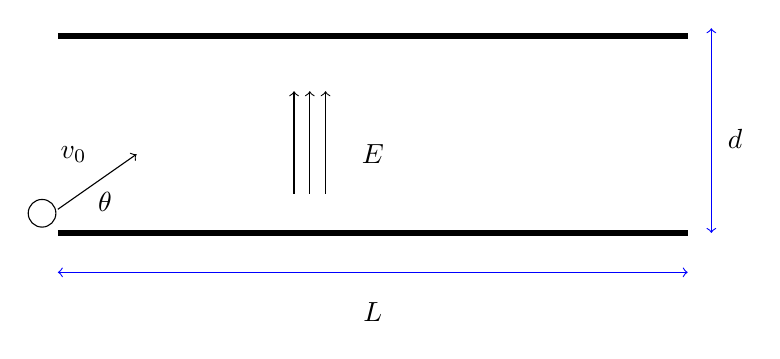
\begin{tikzpicture}
    	\draw [line width=2pt](0,0) -- (8,0);
    	\draw [line width=2pt](0,2.5) -- (8,2.5);
        \draw [->](3,0.5)--(3,1.8);
        \draw [->](3.2,0.5)--(3.2,1.8);
        \draw [->](3.4,0.5)--(3.4,1.8);
        \draw [->](0,0.3)--(1,1);
        \draw (-0.2,0.25) circle [radius=5pt];
        \draw [<->,blue] (0,-0.5)--(8,-0.5);
        \draw [<->,blue] (8.3,0)--(8.3,2.6);
        \node at (4,1) {$E$};
        \node at (0.6,0.4) {$\theta$};
        \node at (0.2,1){$v_0$};
        \node at (4,-1) {$L$};
        \node at (8.6,1.2){$d$};
    \end{tikzpicture}
    \end{center}

    \begin{minipage}{0.6\textwidth}
    \item Suatu bola bermassa $m$ digantungkan dengan sutas tali pada suatu bidang bermuatan yang terdistribusi merata (non-konduktor). Bola bermuatan $q$ dan bola seimbang ketika tali membentuk sudut $\theta$ bidang dengan vertikal. Hitung kerapatan muatan bidang!
    \end{minipage}
    \hfill
    \begin{minipage}{0.25\textwidth}
    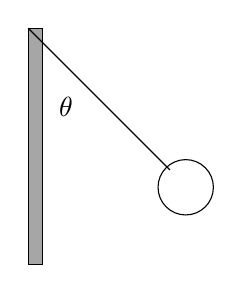
\begin{tikzpicture}
        \filldraw[fill=gray!70] (0,0) rectangle (0.18,3);
        \draw (1.8,1.2)--(0,3);
        \draw (2,0.98) circle [radius=10pt];
        \node at (0.48,2) {$\theta$};
    \end{tikzpicture}
    \end{minipage}

    \item Suatu elektron $115keV$ ditembakkan ke arah suatu lembaran plastik yang mempunyai kerapatan permukaan $-2.08\mu C/m^{2}$. Dari jarak berapa elektron harus ditembakkan agar kecepatan saat menyentuh lembaran itu nol?
\end{enumerate}